
\section{Quarta Questão (9 pts)}

\subsection{Análise Analítica}

\numberwithin{equation}{section}
\numberwithin{figure}{section}

De modo parecido à modelagem do Prolema 3, temos que partir das equações de Navier-Stokes e 
da equação de conservação da massa, assumindo escoamento incompressível. 
Podemos fazer as seguintes simplificações:

\begin{itemize}
    \item Estamos modelando a geometria apenas em duas dimensões $x$ e $y$: $w = 0$ e derivadas em relação a $z$ nulas.
    \item Gravidade atua apenas na componente $y$: $g_x = g_z = 0$
    \item Regime permanente: derivadas em relação a $t$ nulas
\end{itemize}

Com essas simplificações, temos três equações que modelam o problema

\begin{equation}\label{eq:Q4NS1}
        \rho\left(u\diffp{u}{x} + v\diffp{u}{y}\right)
         = \diffp{p}{x} + \mu \left(\diffp[2]{u}{x} + \diffp[2]{u}{y}\right)
\end{equation}

\begin{equation}\label{eq:Q4NS2}
        \rho\left(u\diffp{v}{x} + v\diffp{v}{y}\right)
         = \rho g_y - \diffp{p}{y} + \mu \left(\diffp[2]{v}{x} + \diffp[2]{v}{y}\right)
\end{equation}

\begin{equation}\label{eq:MassConservationQ4}
    \diffp{u}{x} + \diffp{v}{y} = 0
\end{equation}

Conforme as equações \eqref{eq:Q4NS1}, \eqref{eq:Q4NS2} e \eqref{eq:MassConservationQ4},
temos que as velocidades horizontal $u$ e vertical $v$ são funções de duas variáveis: $x$ e $y$.
A injeção de ar pela face sul é de baixo para cima, logo temos efeito da gravidade no fluido,
representada pelo termo $\rho g_y$ em \eqref{eq:Q4NS2}. 

Os gradientes de pressão na direçao $x$ e $y$
não foram informados no enunciado do problema, mas podemos assumir que existem gradientes 
causando os movimentos do fluido em ambas direçoes $x$ e $y$. Nessa interpretação, usamos a analogia
que gradientes de pressão causam movimento de fluidos da mesma forma que gradientes de potencial
elétrico (tensão) geram fluxo de corrente elétrica. 

Uma vez identificado as equações diferenciais que modelam o problema, temos que determinar
as condições de contorno. Na face oeste, temos

\begin{equation}\label{eq:q4WestBoundary}
    \begin{cases}
        u(0, y) = 0.06 \un{m/s}, & 0 \leq y \leq 1 \un{cm} \\
        v(0, y) = 0 \un{m/s}, & 0 \leq y \leq 1 \un{cm} \\
    \end{cases}
\end{equation}

Na face leste temos sáida, que significa escoamento plenamente
desenvolvido, ou seja, derivadas espaciais nulas.

\begin{equation}\label{eq:q4EastBoundary}
    \begin{cases}
        \diffp{u}{x} = \diffp{u}{y} = 0, & x = 20 \un{cm}, 0 \leq y \leq 1 \un{cm}  \\
        \diffp{v}{x} = \diffp{v}{y} = 0, & x = 20 \un{cm}, 0 \leq y \leq 1 \un{cm} \\
    \end{cases}
\end{equation}

Na face sul temos uma região da parede que é fixa, e outra que é porosa com injeção
de ar de baixo para cima. Assim, temos

\begin{equation}\label{eq:q4SouthBoundary}
    \begin{cases}
        u(x, 0) = 0, & 0 \leq x \leq 20 \un{cm}  \\
        v(x, 0) = 0, & 0 \leq x \leq 10 \un{cm}  \\
        v(x, 0) = 0.02 \un{m/s}, & 10 \leq x \leq 20 \un{cm}  \\
    \end{cases}
\end{equation}

Na face norte temos condições de contorno simétricas à face sul. Note que na face
sul é injeção de ar, e na face norte é sucção de ar, de modo que a direção e sentido
de $v$ em ambas faces é a mesma.

\begin{equation}\label{eq:q4NorthBoundary}
    \begin{cases}
        u(x, 1 \un{cm}) = 0, & 0 \leq x \leq 20 \un{cm}  \\
        v(x, 1 \un{cm}) = 0, & 0 \leq x \leq 10 \un{cm}  \\
        v(x, 1 \un{cm}) = 0.02 \un{m/s}, & 10 \leq x \leq 20 \un{cm}  \\
    \end{cases}
\end{equation}

Finalmente, o problema é modelado matematicamente pelas equações diferenciais parciais
\eqref{eq:Q4NS1}, \eqref{eq:Q4NS2} e \eqref{eq:MassConservationQ4}, com as condições de 
contorno especificadas em \eqref{eq:q4WestBoundary}, \eqref{eq:q4EastBoundary}, 
\eqref{eq:q4SouthBoundary} e \eqref{eq:q4NorthBoundary}.

\subsection{Análise Numérica}

Ao contrário dos Problemas 1, 2 e 3, discretizar as equações diferenciais \eqref{eq:Q4NS1}, \eqref{eq:Q4NS2} e \eqref{eq:MassConservationQ4}
e desenvolver um programa para analisar numericamente seria bastante trabalhoso. Assim, 
usamos o software gratuito CFD Studio para obter a distribuição de velocidades. 

As configurações usadas no software foram as seguintes:

\begin{itemize}
    \item Tipo de malha utilizado: malha cartesiana, com 10 divisões na vertical e 20 na horizontal
    \item Esquema de interpolação: UDS
    \item Algoritmo de acoplamento pressão velocidade (P-V): simplec
    \item Coeficiente de sub-relaxação da pressão: 1.00
    \item Pressão de referência: $0 \un{N/m}$
    \item Local de imposição de pressão de referência: Malha $i = 19$, $j = 0$, no canto inferior da face leste
    \item Número de iterações necessárias até convergir: 5000
    \item Solver utilizado: Gauss Seidel
\end{itemize}

As demais configurações do software foram as padrões para escoamento sem transferência de calor,
seguindo os passos do Assistente de Problema CFD.

As condições iniciais são $u = v = 0$ em todo o domínio pois o regime de escoamento é permanente.
O material selecionado foi ar, com propriedades de viscosidade $\mu=1.85 \cdot 10^{-5} \un{ kg m$^{-1}$ s$^{-1}$}$ e
massa específica $\rho=1.161 \un{kg m$^{-3}$}$.

As condições de contorno \eqref{eq:q4WestBoundary}, \eqref{eq:q4EastBoundary}, 
\eqref{eq:q4SouthBoundary} e \eqref{eq:q4NorthBoundary} podem facilmente ser inseridas 
no software através da interface gráfica. 

Uma vez inseridos todas essas condições de contorno e configurações, a Figura \ref*{fig:convergencia}
exibe a convergência da simulação realizada.

\begin{figure}[h!]
    \caption{Convergência da simulação no CFD Studio.}
    \label{fig:convergencia}
    \centering
    \centerline{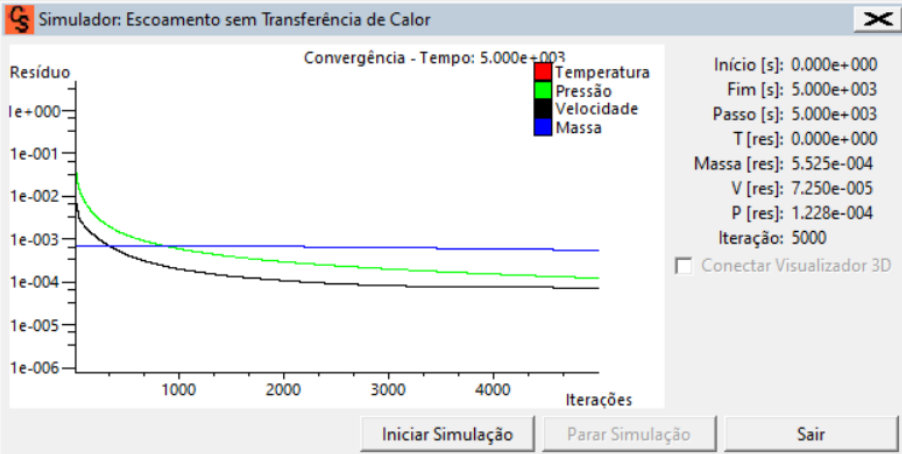
\includegraphics[scale=0.45]{convergencia.png}}
    \par{Fonte: elaboração própria.}
\end{figure}

Como visto na Figura \ref*{fig:convergencia}, a configuração selecionada atingiu uma boa  
convergência de velocidade, pressão e massa. A Figura \ref*{fig:velocidades} exibe a 
distibuição do campo de velocidades simulado. Os vetores da imagem foram escalados por um fator
3 para melhorar a visualização.

\begin{figure}[h!]
    \caption{Distribuição de velocidades no problema, obtida com o CFD Studio.}
    \label{fig:velocidades}
    \centering
    \centerline{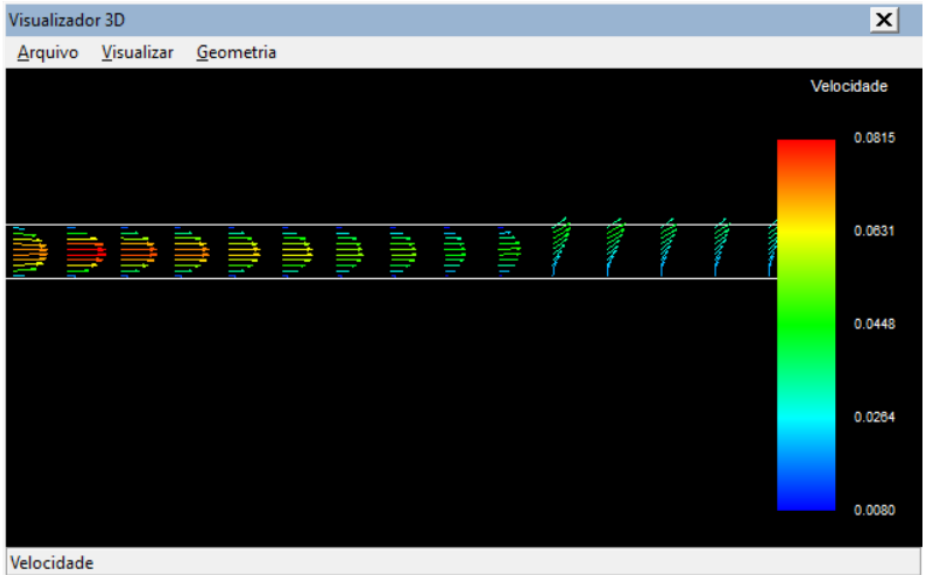
\includegraphics[scale=0.45]{velocidades.png}}
    \par{Fonte: elaboração própria.}
\end{figure}

A distribuição na Figura \ref*{fig:velocidades} é condizente com o esperado fisicamente. Quando 
o fluido de alta velocidade entra no espaço entra as placas, o escoamento apresenta um perfil
parabólico, e conforme o fluido avança no espaço entre as placas na direção $x$ a 
velocidade vai se reduzindo. Ao atingir o centro do tubo ($x = 10 \un{cm}$), a injeção
vertical de ar através da face sul porosa deforma o perfil até então parabólico do escoamento.
De fato, para $x \geq 10 \un{cm}$, temos uma distribuição de velocidades como uma parábola deslocada
para cima, resultado da força para cima exercida pelo ar injetado.

A Figura \ref*{fig:pressao} exibe a distribuição de pressão ao longo do tubo. Note que fixamos a pressão de referência 
em zero no canto inferior direito da geometria na configuração da pressão de referência.
Além disso, temos que a pressão é maxima no ponto de entrada do fluido de alta velocidade,
o que também é conforme o esperado fisicamente.

\begin{figure}[h!]
    \caption{Distribuição de pressão no problema, obtida com o CFD Studio.}
    \label{fig:pressao}
    \centering
    \centerline{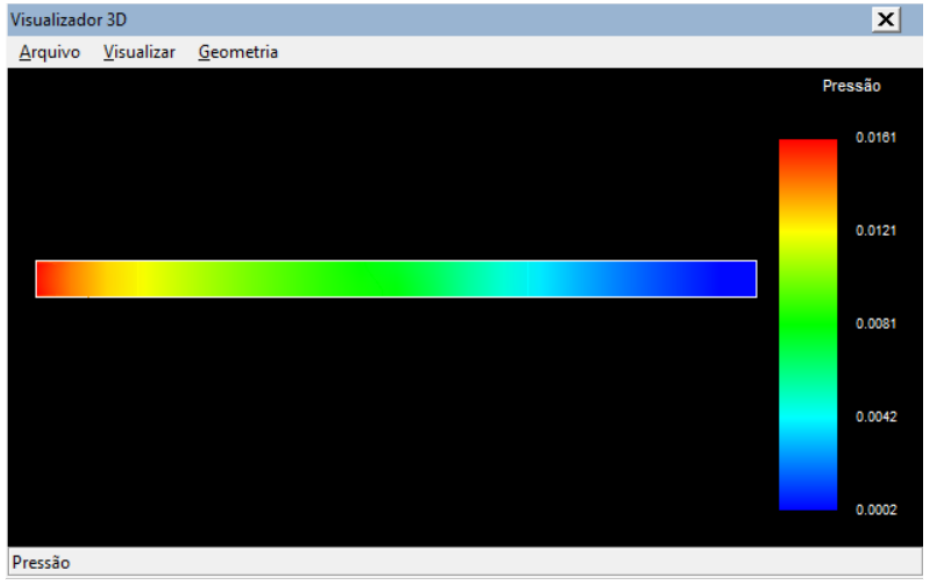
\includegraphics[scale=0.45]{pressao.png}}
    \par{Fonte: elaboração própria.}
\end{figure}

A Figura \ref*{fig:velocidadesLinha} mostra o perfil de velocidades ao longo de duas retas
verticais no tubo, a primeira na linha $i = 4$ (quinta divisão horizontal), antes da injeção 
de ar, e a segunda na linha em $i = 15$ (décima sexta divisão horizontal), que é depois
da injeção de ar.

\begin{figure}[h!]
    \caption{Perfil de velocidades ao longo linhas verticais $i = 4$ e $i = 15$ no tubo.}
    \label{fig:velocidadesLinha}
    \centering
    \centerline{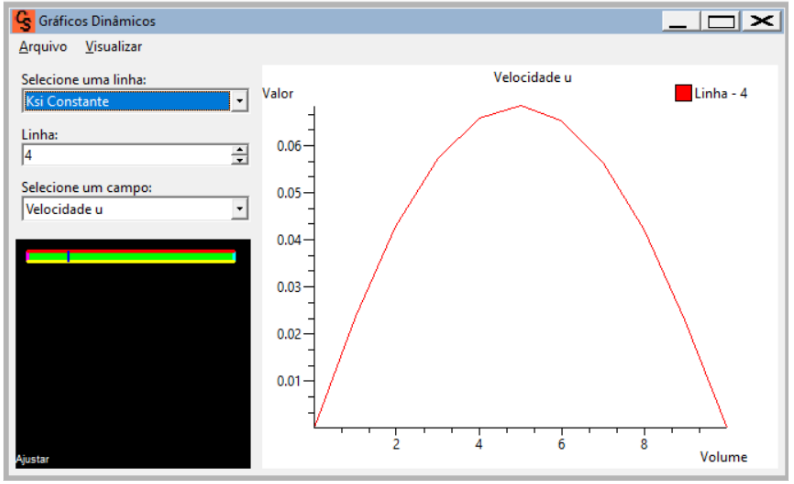
\includegraphics[scale=0.5]{velocidadeLinha4.png}}
    \centerline{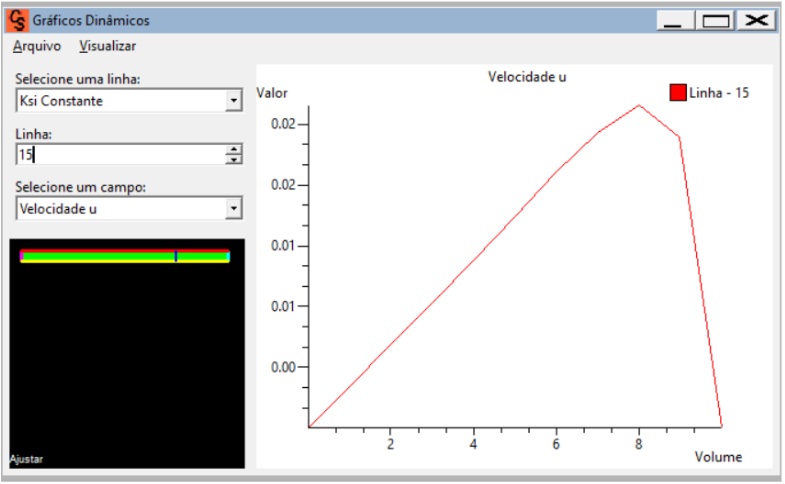
\includegraphics[scale=0.5]{velocidadeLinha15.png}}
    \par{Fonte: elaboração própria.}
\end{figure}

Os gráficos da Figura \ref*{fig:velocidadesLinha} reforçam a análise feita com o campo vetorial da velocidade 
na Figura \ref*{fig:velocidades}. Após a injeção de ar, o perfil parabólico do escoamento é deformado
para cima.

A última análise que podemos fazer com o CFD Studio é o teste de malhas. Os resultados acima 
foram obtidos com uma malha $20 \times 10$, totalizando 200 nós. Vamos refazer a simulação com
uma malha $100 \times 50$, com 5000 nós, para verificar o impacto do refinamento da malha nos resultados.
A distribuição de velocidades obtida com essa malha foi está exibida na 

\begin{figure}[h!]
    \caption{Perfil de velocidades obtido com a malha $100 \times 50$.}
    \label{fig:velocidadeFina}
    \centering
    \centerline{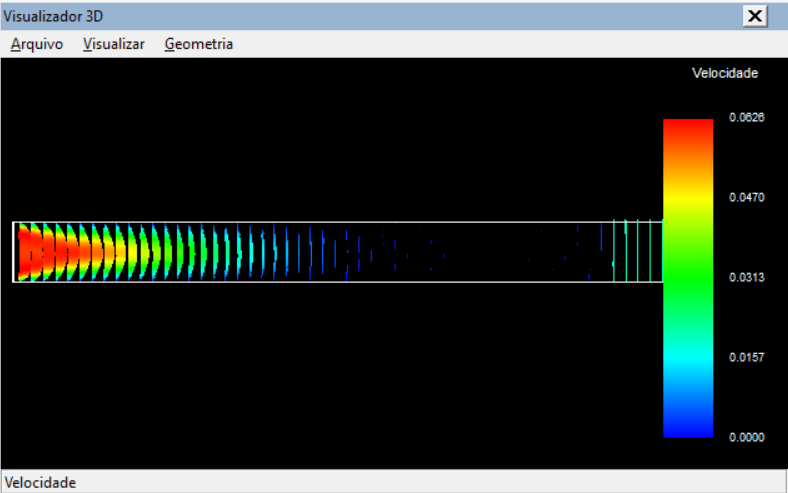
\includegraphics[scale=0.5]{velocidadeFina.png}}
    \par{Fonte: elaboração própria.}
\end{figure}

Comparando as Figuras  \ref*{fig:velocidades} e \ref*{fig:velocidadeFina}, temos que as velocidades
calculadas na entrada e no início da região porosa são similares. A principal diferença observada
é que, na malha $100 \times 50$, o escoamento praticamente se encerrou em $x = 5 \un{cm}$, sendo retomado
apenas quando ocorre a injeção de ar a partir de $x \geq 10 \un{cm}$. Por outro lado,
na entrada do tubo, temos um perfil muito mais detalhado da distribuição de velocidades quando o ar
inicialmente entra no espaço entre as placas.

É importante destacar que a simulação feita na Figura \ref*{fig:velocidadeFina} foi com apenas 1000 iterações,
ao passo que a iteração da Figura  \ref*{fig:velocidades} teve 5000. Isso foi feito pois, com o aumento no número 
de nós, o tempo gasto por iteração aumentou consideravelmente. Para executar as 1000 iterações na nova malha, foi gasto quase
2 minutos.



